\documentclass[11pt,a4paper]{article}

\usepackage[utf8]{inputenc}
\usepackage[T1]{fontenc}
\usepackage{lmodern}
\usepackage[margin=1in]{geometry}

\usepackage{graphicx}
\usepackage{booktabs}
\usepackage{float}
\usepackage{xcolor}
\usepackage{hyperref}
\usepackage{enumitem}
\usepackage{subcaption}

\hypersetup{
    colorlinks=true,
    linkcolor=blue!60!black,
    urlcolor=blue!60!black,
}

\title{AI Agent Code Coverage: Ablation Study\\
\large Prompt, Knowledge, Model, and Framework Effects on AI-Generated Tests}
\author{Mark Pollack}
\date{March 2026 --- DevNexus}

\begin{document}
\maketitle

%% ==================================================================
\section{Setup}

\textbf{Task}: Given a Spring Boot project with production code and \emph{no tests},
generate a JUnit test suite targeting $\geq$80\% line coverage.

\textbf{Dataset}: 5 Spring Getting Started guides (trivial, 2--3 classes) +
Spring Pet Clinic (complex, 15+ classes, 4 layers).

\textbf{Notation}: \texttt{Agent:Model} --- e.g., \texttt{CC:Sonnet} = Claude Code CLI
running Claude Sonnet 4.6; \texttt{Loopy:Haiku} = Loopy framework (Spring AI agent)
running Claude Haiku 4.5.

\textbf{Variants tested} --- two axes of variation:

\begin{table}[H]
\centering
\small
\begin{tabular}{@{}lllp{6cm}@{}}
\toprule
\textbf{Agent:Model} & \textbf{Prompt} & \textbf{Knowledge} & \textbf{What it tests} \\
\midrule
CC:Sonnet (naive)     & v0-naive    & none     & Baseline --- minimal instructions \\
CC:Sonnet (hardened)  & v1-hardened & none     & Does prompt quality matter? \\
CC:Sonnet (+3 KB)     & v2-with-kb  & 3 files  & Does curated knowledge help? \\
CC:Sonnet (+full KB)  & v2-with-kb  & full KB  & Does more knowledge help more? \\
CC:Sonnet (two-phase) & v3-explore+act & full KB & Does structured execution help? \\
CC:Sonnet (+SAE)      & v1-hardened+SAE & none & Does pre-computed analysis help Sonnet? \\
CC:Haiku              & v1-hardened & none     & Can a cheap model match Sonnet? \\
CC:Haiku (+SAE)       & v1-hardened+SAE & none & Does pre-computed analysis help Haiku? \\
Loopy:Haiku           & v1-hardened & none     & Does the framework matter? \\
Loopy:Sonnet          & v1-hardened & none     & Does Sonnet fix Loopy's quality gap? \\
Loopy:Qwen3           & v1-hardened & none     & Can a free local model do the job? \\
\bottomrule
\end{tabular}
\end{table}

\textbf{Scoring}: 4-tier automated judge cascade ---
build success (T0), coverage preservation (T1),
coverage improvement + golden test similarity (T2),
LLM practice adherence across 6 criteria (T3).

%% ==================================================================
\section{Results at a Glance}

\input{tables/variant-comparison}

\input{tables/cost-analysis}

%% ==================================================================
\section{Key Findings}

\subsection{Finding 1: Prompt Engineering Is the Biggest Lever}

\begin{figure}[H]
\centering
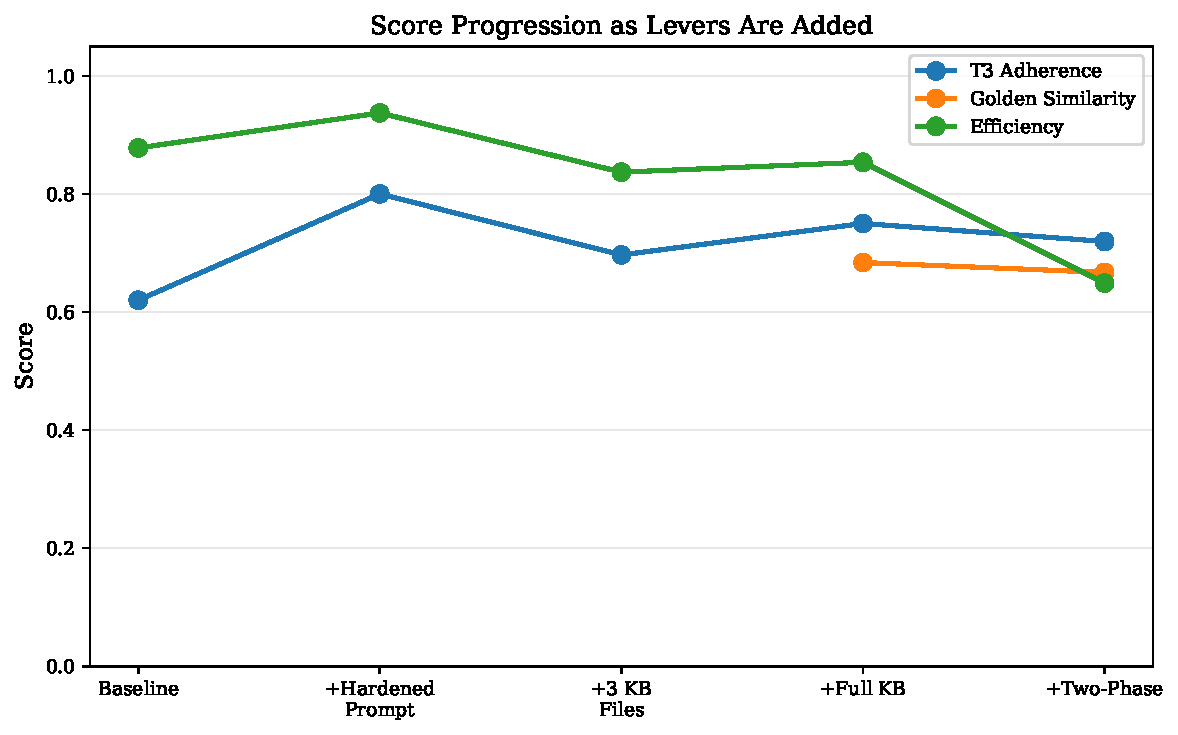
\includegraphics[width=0.8\textwidth]{figures/growth-story.pdf}
\caption{Score progression as levers are added. The jump from naive to
hardened prompt is the dominant improvement.}
\end{figure}

CC:Sonnet (hardened) delivers the best quality: T3=0.81, 100\% pass rate,
\$1.39/item. Knowledge injection and two-phase execution add cost without
measurable benefit on simple targets.

\subsection{Finding 2: Model Is the Quality Gate, Framework Is the Cost Gate}

Quality depends on model capability. Cost depends on framework engineering.
These are \textbf{independent axes}.

\begin{table}[H]
\centering
\small
\begin{tabular}{@{}llrrrl@{}}
\toprule
\textbf{Agent:Model} & \textbf{Framework} & \textbf{T3} & \textbf{Cost} & \textbf{Input Tokens} & \textbf{Passed} \\
\midrule
CC:Haiku         & Claude Code & 0.40 & \$0.45  & 300         & No \\
Loopy:Haiku      & Loopy (no compaction) & 0.49 & \$2.55  & 18,336,594  & No \\
CC:Sonnet        & Claude Code & 0.70 & \$0.92  & ---         & Yes \\
Loopy:Sonnet     & Loopy (with compaction) & 0.73 & \$2.72  & 854,353     & Yes \\
\bottomrule
\end{tabular}
\caption{gs-accessing-data-jpa: same item, same prompt across four agent/model combinations.}
\end{table}

Read the rows: Haiku fails regardless of framework (T3 0.40--0.49, both fail jury).
Sonnet passes regardless of framework (T3 0.70--0.73, both pass jury).
The model determines \emph{whether it works}. The framework determines \emph{what it costs}.

Read the columns: Loopy:Haiku without compaction: 18M input tokens.
Loopy:Sonnet with compaction (threshold 0.3): 854K input tokens ---
a \textbf{21$\times$} reduction. Context compaction closes most of the framework gap,
but Loopy:Sonnet still costs \textbf{3$\times$} more than CC:Sonnet at API rates.

\textit{First Loopy:Sonnet run hit the \$5 cost cap at turn 54 with compaction
threshold 0.5. Lowering to 0.3 (compact at 60K tokens) let it complete at \$2.72.
Compaction tuning matters --- too late and you burn budget on stale context.}

\subsection{Finding 3: There Is a Model Floor}

Both CC:Haiku (T3=0.44) and Loopy:Haiku (T3=0.49) achieve decent
\textbf{coverage} (71--94\%) but fail the quality jury. Common failures:
wrong test annotations (\texttt{@SpringBootTest} everywhere instead of
\texttt{@WebMvcTest}), wrong injection patterns, no edge case tests.
Below the model floor, no amount of framework engineering, knowledge injection,
or prompt tuning helps. Haiku and Qwen3 are below that floor for Spring testing.

\subsection{Finding 4: Knowledge Amplifies Capability}

We built a lightweight \textbf{Stable Analysis Envelope (SAE)} --- a pre-computed
project report generated after compilation that gives the agent: dependency inventory,
component classification (controllers, services, repos, entities), and
\textbf{copy-paste import blocks} with full package names for each test slice.

We iterated the SAE through two versions, then tested each against two models:

\begin{description}[style=nextline, leftmargin=2em]
  \item[SAE v1 (short annotations)]
    Component roles and dependency list only. Tells the agent \emph{what exists}
    but not \emph{how to import it}. Result: the agent still launched
    \texttt{jar tf} commands to discover package names.
  \item[SAE v2 (full import blocks)]
    Adds ready-to-paste import statements for every test slice
    (\texttt{@WebMvcTest}, \texttt{@DataJpaTest}, etc.).
    Result: zero jar exploration --- the agent writes tests immediately.
\end{description}

\begin{table}[H]
\centering
\small
\begin{tabular}{@{}llrrrrl@{}}
\toprule
\textbf{Model} & \textbf{SAE} & \textbf{T3} & \textbf{Cov\%} & \textbf{Cost} & \textbf{jar-inspect} & \textbf{Passed} \\
\midrule
Haiku   & none    & 0.43 & 71.4 & \$0.44 & 0 & No \\
Haiku   & v1      & 0.45 & 71.4 & \$0.39 & 8 & No \\
Haiku   & v2      & 0.35 & 71.4 & \$0.48 & 0 & No \\
\addlinespace
Sonnet  & none    & 0.81 & 85.7 & \$0.83 & --- & Yes \\
Sonnet  & v2      & 0.93 & 71.4 & \$0.92 & 0 & Yes \\
\bottomrule
\end{tabular}
\caption{SAE ablation on gs-rest-service (single item, N=1).
Rows are grouped by model. Haiku with any SAE version still fails the quality jury.
Sonnet with SAE v2: T3=0.93, the highest single-item score in the experiment.}
\end{table}

Three things stand out:

\begin{enumerate}
  \item \textbf{SAE v2 eliminates exploratory waste.} Zero \texttt{jar tf}
        calls --- the agent writes tests immediately instead of probing JARs.
  \item \textbf{SAE amplifies capable models.} Sonnet + SAE: T3 jumps from
        0.81 to 0.93. Same model, same prompt, just better context.
  \item \textbf{SAE cannot lift weak models.} Haiku + SAE v2: T3 \emph{drops}
        to 0.35. The information is all there; Haiku can't use it correctly.
\end{enumerate}

\textit{Implication}: pre-computed analysis is both an efficiency lever
(fewer wasted tool calls) and a quality lever --- but only when paired with
a model above the capability floor. Knowledge amplifies capability;
it cannot create it.

\subsection{Finding 5: Local Models Are Not Ready}

Loopy:Qwen3 (Qwen3-Coder 30B via LM Studio) scored T3=0.30 with 0\% pass rate.
Even with 300 turns and 45-minute timeout, it couldn't write a single
working test for the simplest project. It spent turns reading files
and writing todo lists instead of writing tests.

\subsection{Finding 6: Partial Knowledge Costs More Than Full or None}

\begin{figure}[H]
\centering
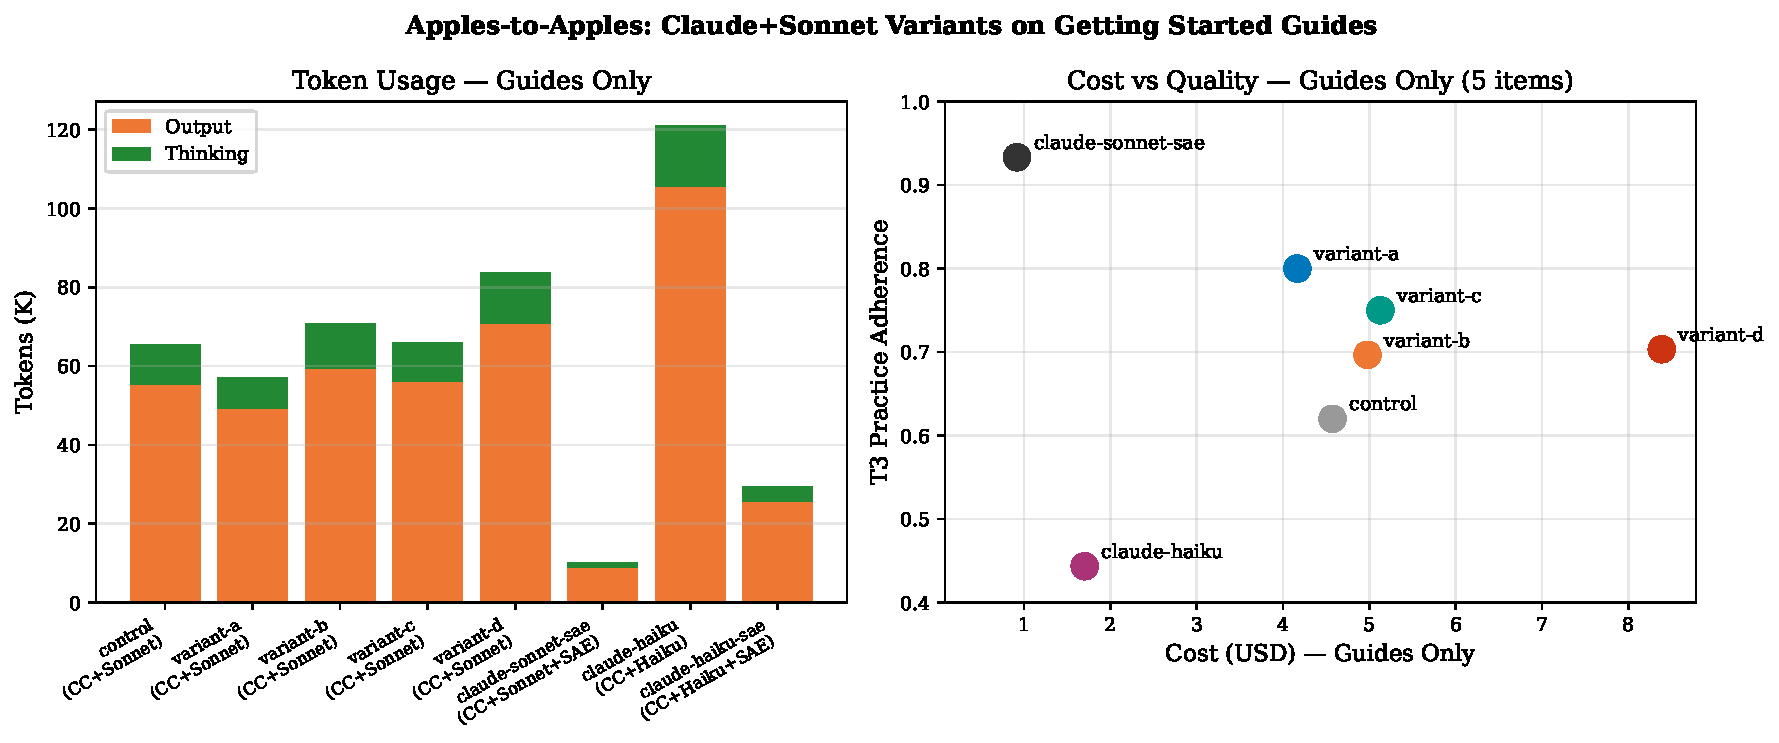
\includegraphics[width=0.9\textwidth]{figures/guides-only-comparison.pdf}
\caption{Guides-only comparison (apples-to-apples, 5 items).
CC:Sonnet (+3 KB) uses more tokens than (+full KB) --- partial knowledge triggers
exploratory \texttt{jar tf} inspection of Spring Boot JARs to fill gaps.}
\end{figure}

\subsection{Finding 7: Two-Phase Costs 2$\times$ for No Gain}

\begin{figure}[H]
\centering
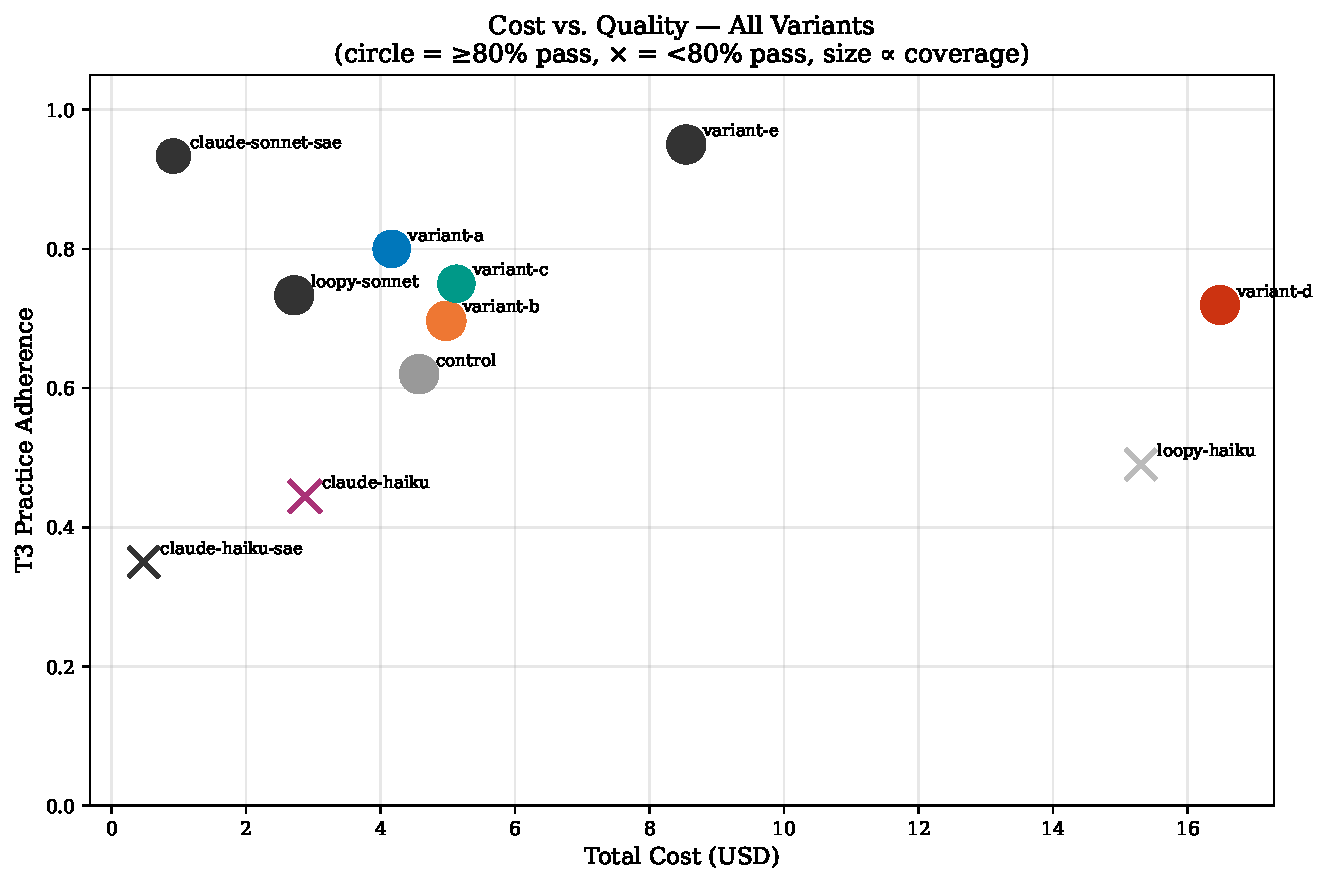
\includegraphics[width=0.75\textwidth]{figures/cost-quality-all.pdf}
\caption{Cost vs.\ quality across all variants.
CC:Sonnet (+SAE) is the new efficient frontier (T3=0.93, \$0.92).
$\circ$ = $\geq$80\% pass, $\times$ = $<$80\% pass, size $\propto$ coverage.}
\end{figure}

%% ==================================================================
\section{Agent Behavior}

\subsection{Token Consumption}

\begin{figure}[H]
\centering
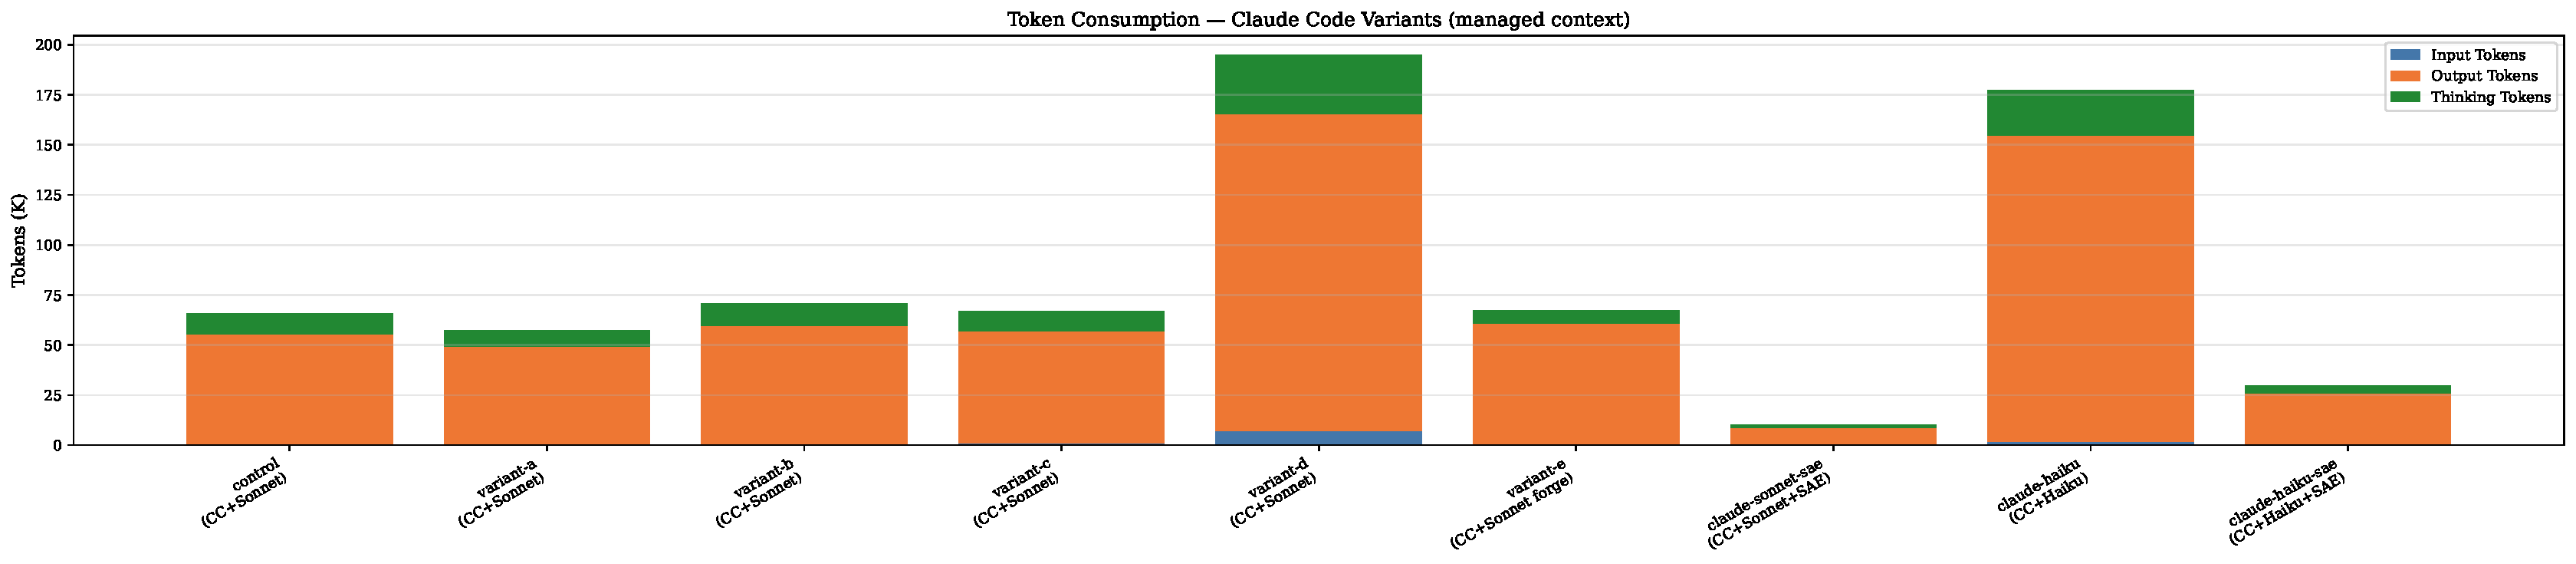
\includegraphics[width=0.85\textwidth]{figures/token-burn-claude.pdf}
\caption{Token consumption --- Claude Code variants. Context is managed by the CLI
(compaction, summarization). Two-phase variant has the highest thinking tokens.}
\end{figure}

\begin{figure}[H]
\centering
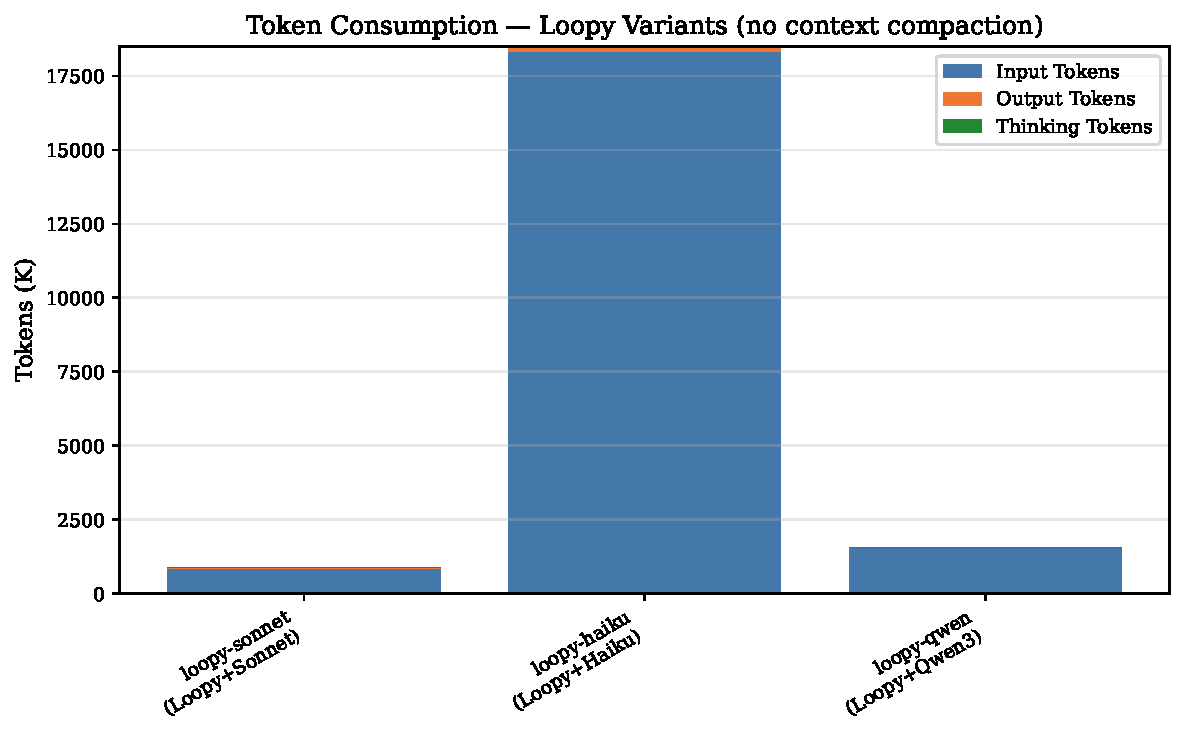
\includegraphics[width=0.85\textwidth]{figures/token-burn-loopy.pdf}
\caption{Token consumption --- Loopy variants (note different Y scale).
Without context compaction, input tokens grow monotonically --- every prior
tool result is re-sent on each turn. This is the dominant cost driver.}
\end{figure}

\subsection{Tool Usage Patterns}

\begin{figure}[H]
\centering
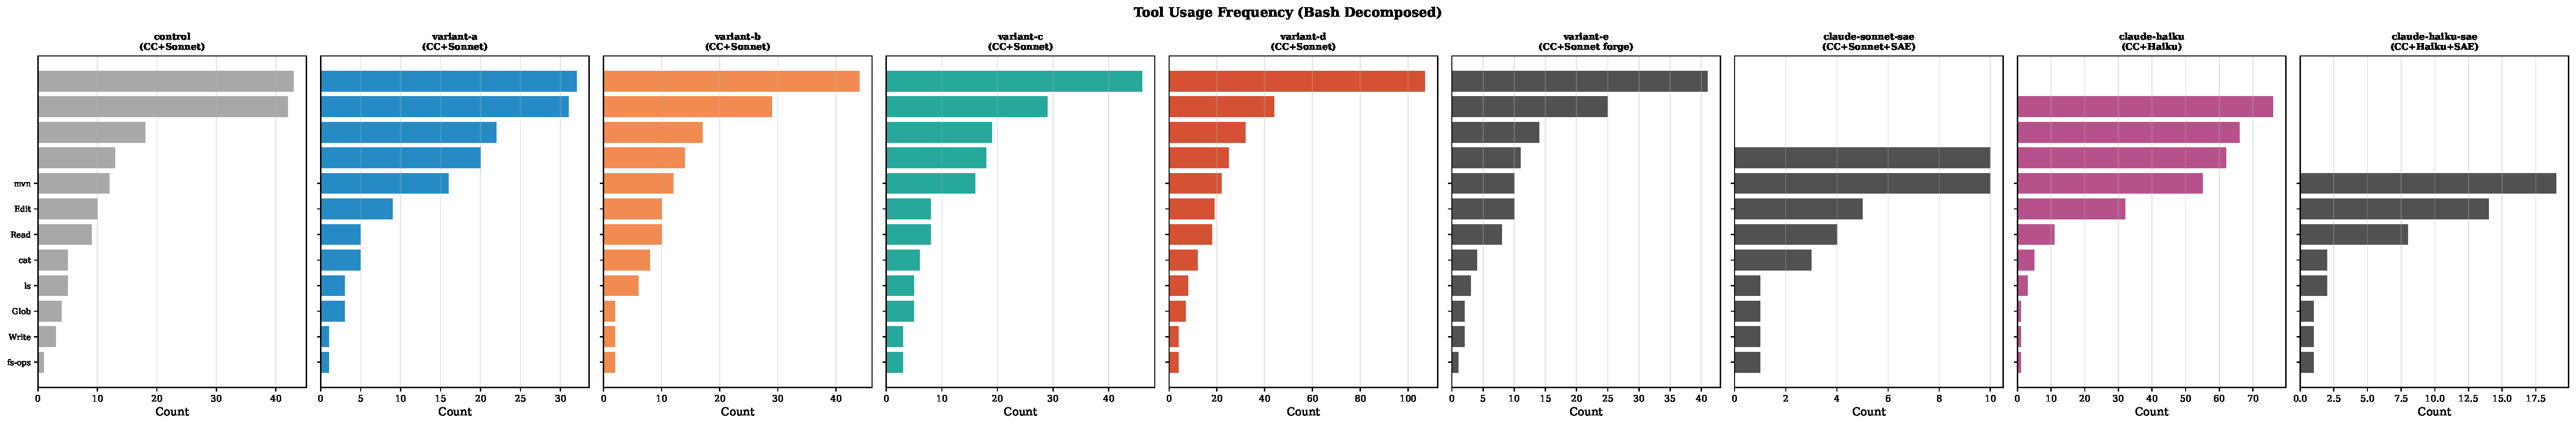
\includegraphics[width=\textwidth]{figures/tool-usage-frequency.pdf}
\caption{Tool call frequency per variant (bash decomposed to actual utilities).
\texttt{jar-inspect} = \texttt{jar tf} commands probing Spring Boot JARs in
\texttt{\textasciitilde/.m2} to discover test annotations.
Knowledge-injected variants need fewer jar inspections.}
\end{figure}

\subsection{Execution Timelines}

\begin{figure}[H]
\centering
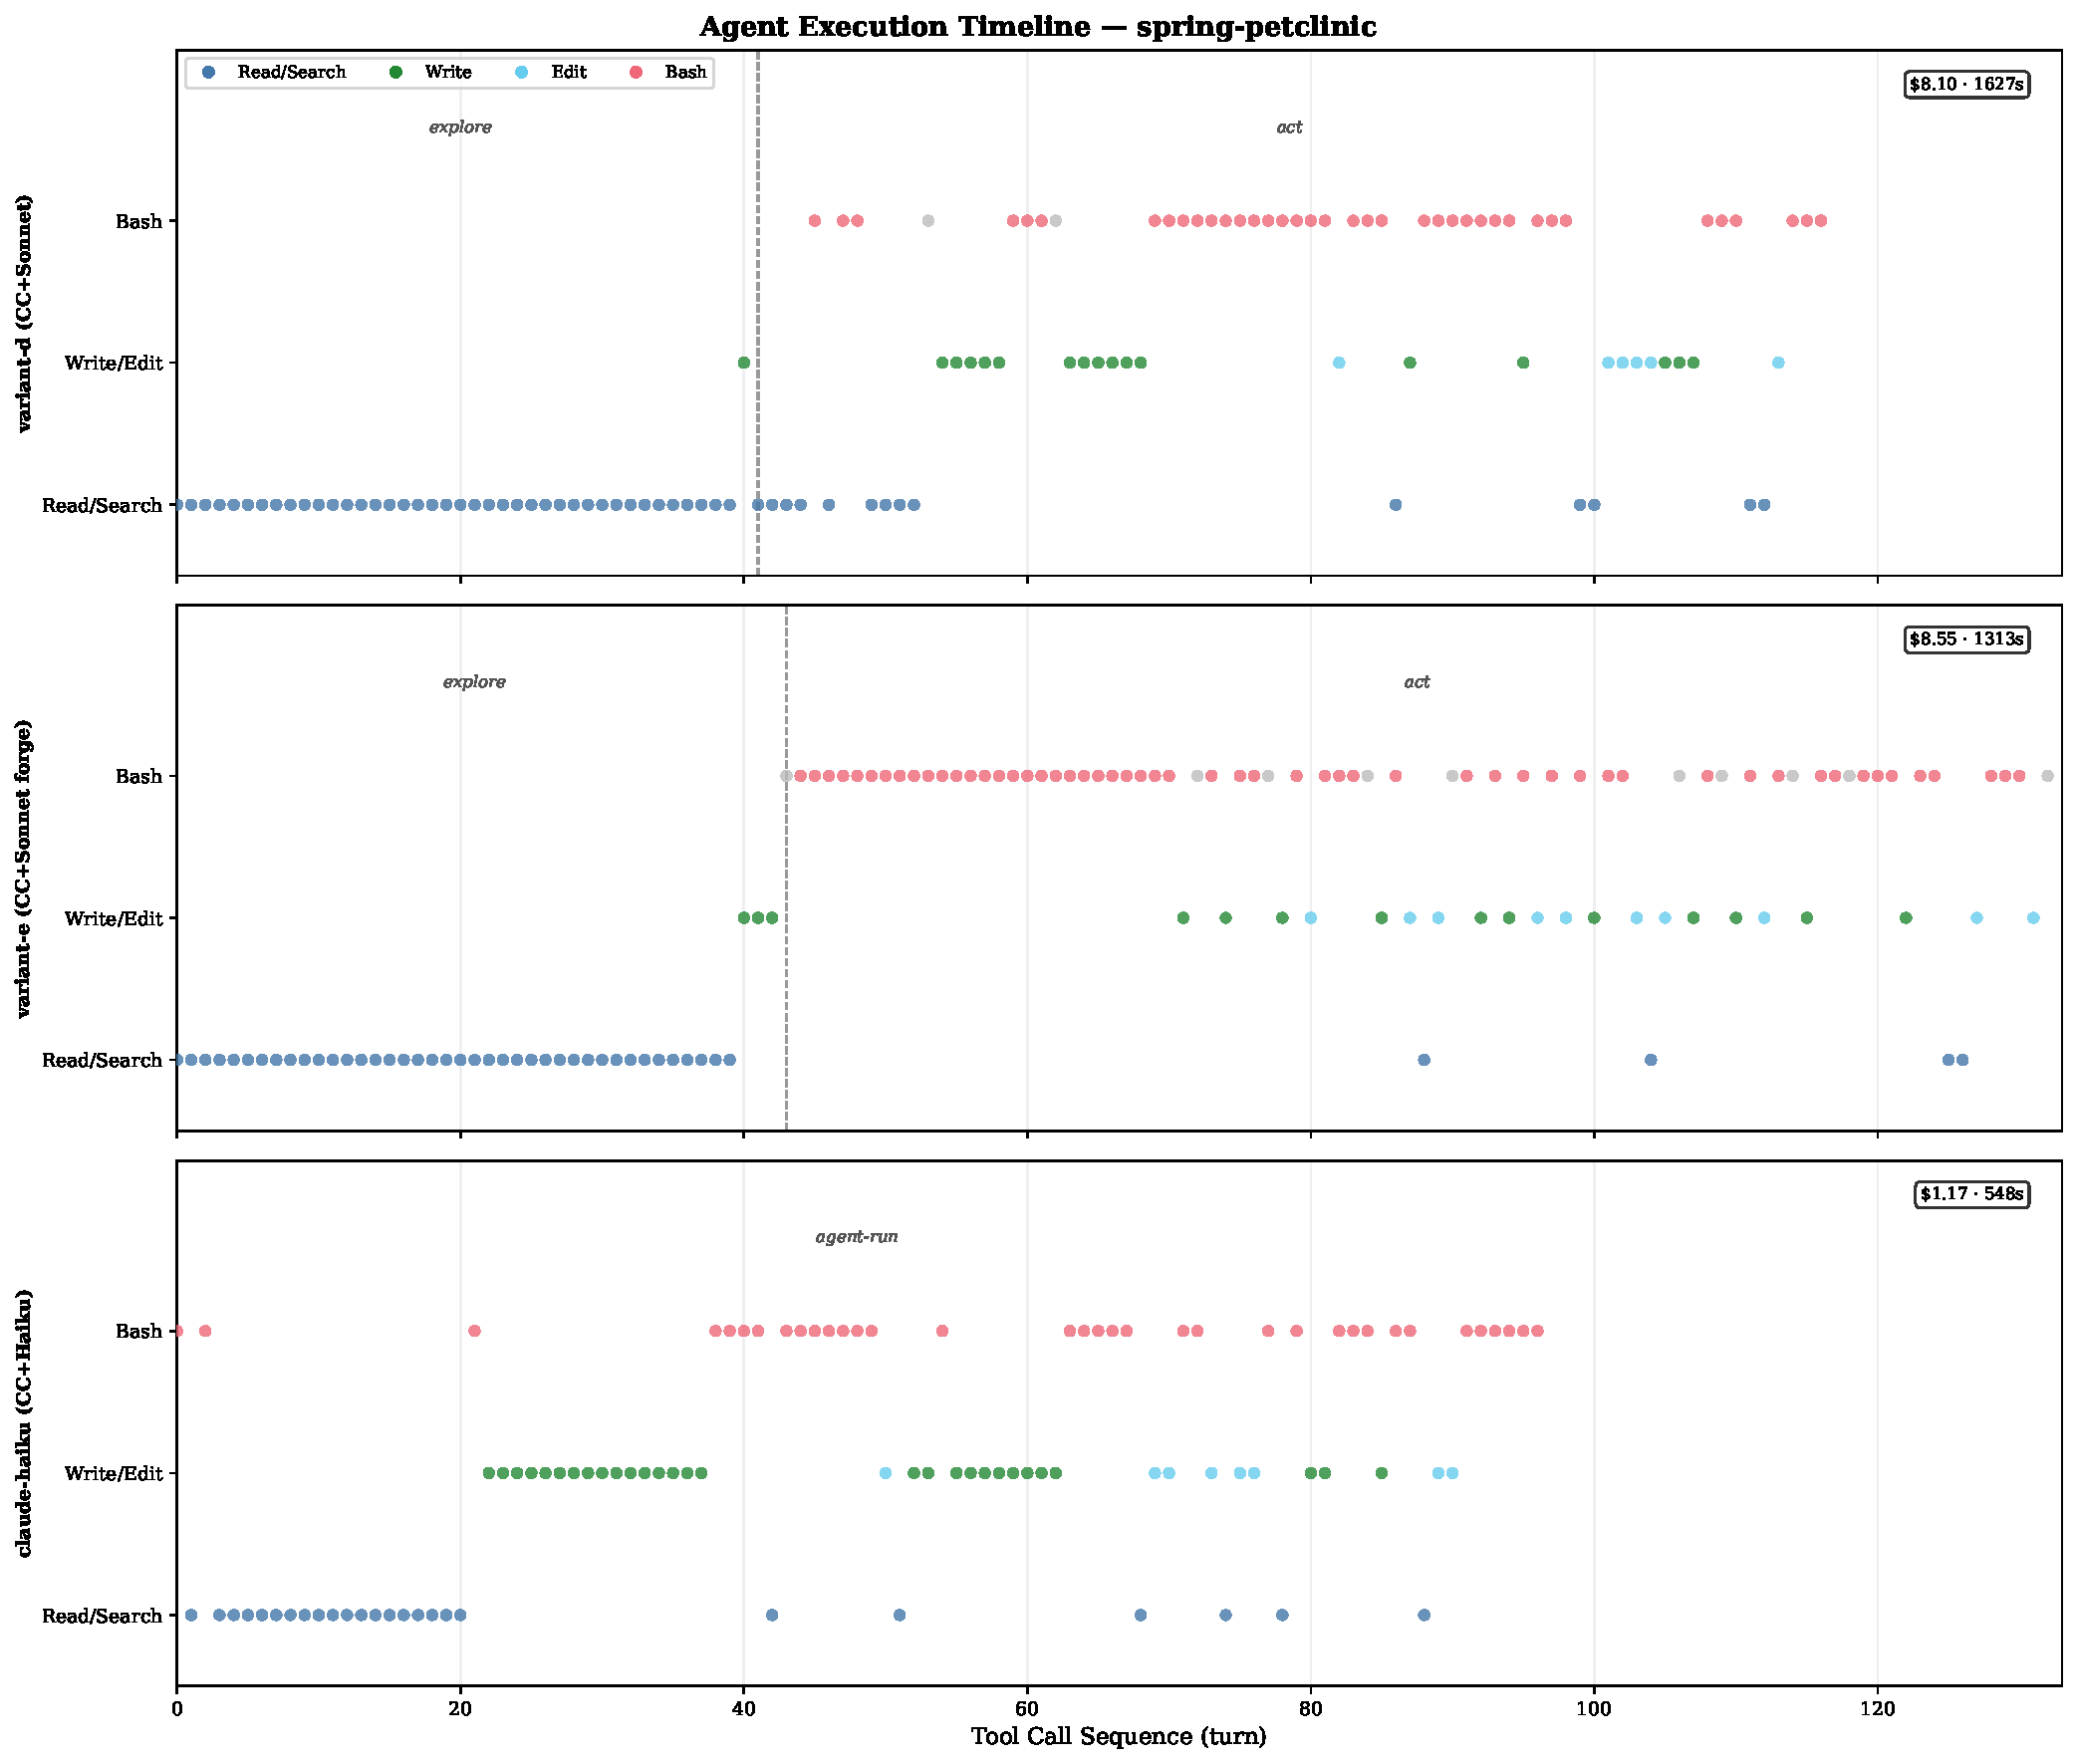
\includegraphics[width=\textwidth]{figures/agent-timeline-petclinic.pdf}
\caption{Agent execution timeline --- Pet Clinic. Each dot is a tool call.
Shared X axis shows relative effort across variants.}
\end{figure}

\begin{figure}[H]
\centering
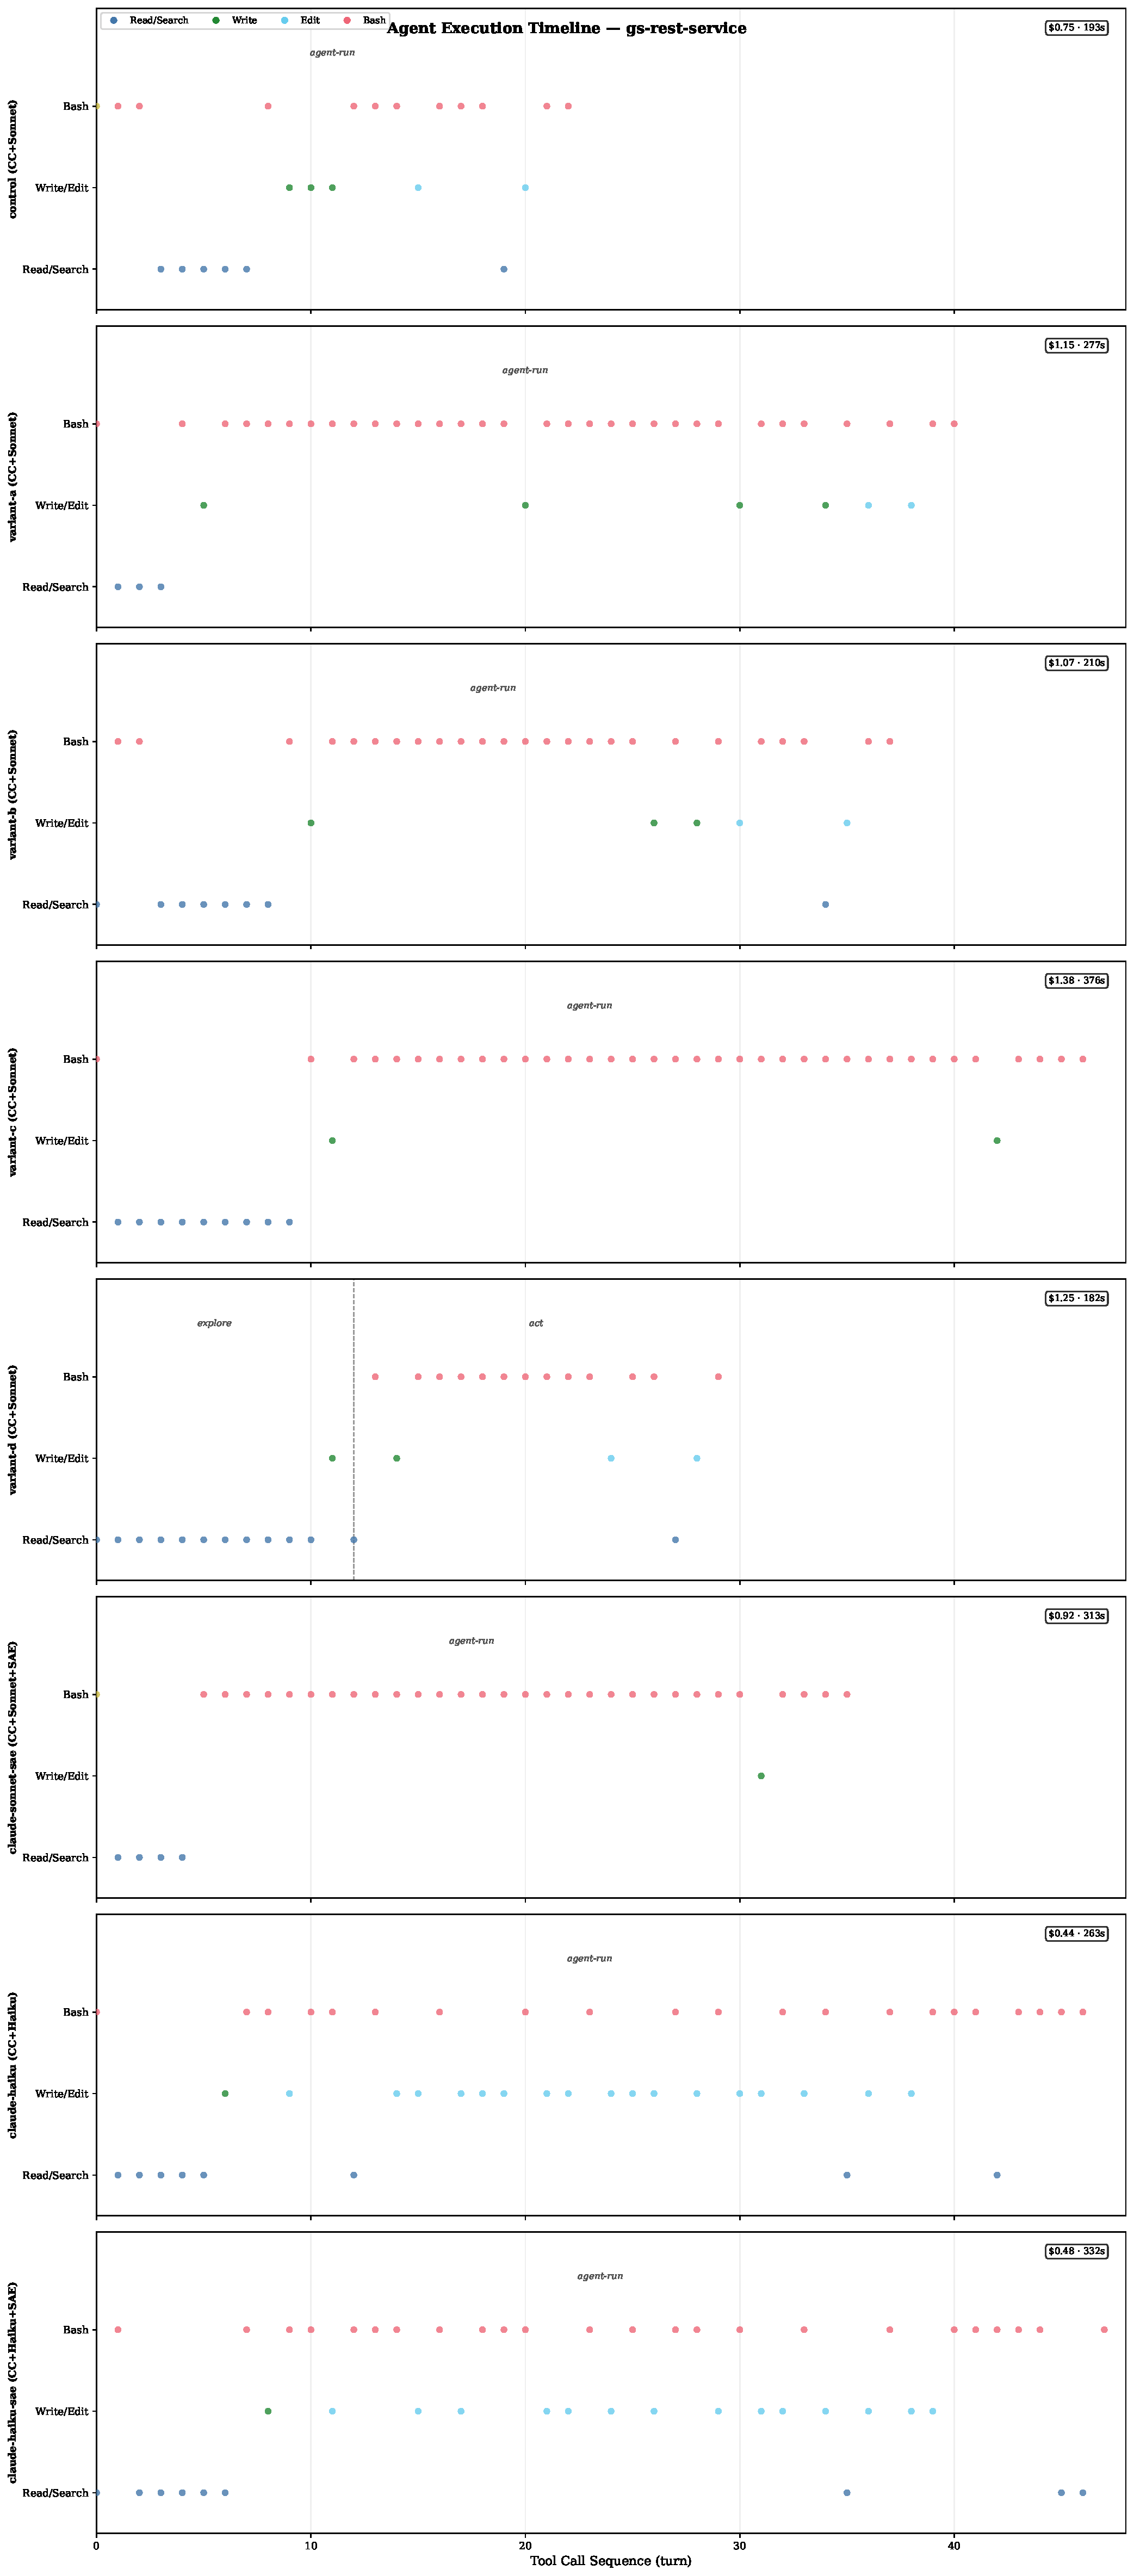
\includegraphics[width=\textwidth]{figures/agent-timeline-rest-service.pdf}
\caption{Agent execution timeline --- gs-rest-service (simplest item).
Much shorter sequences; simple projects don't discriminate between variants.}
\end{figure}

%% ==================================================================
\section{Per-Item Breakdown}

\begin{figure}[H]
\centering
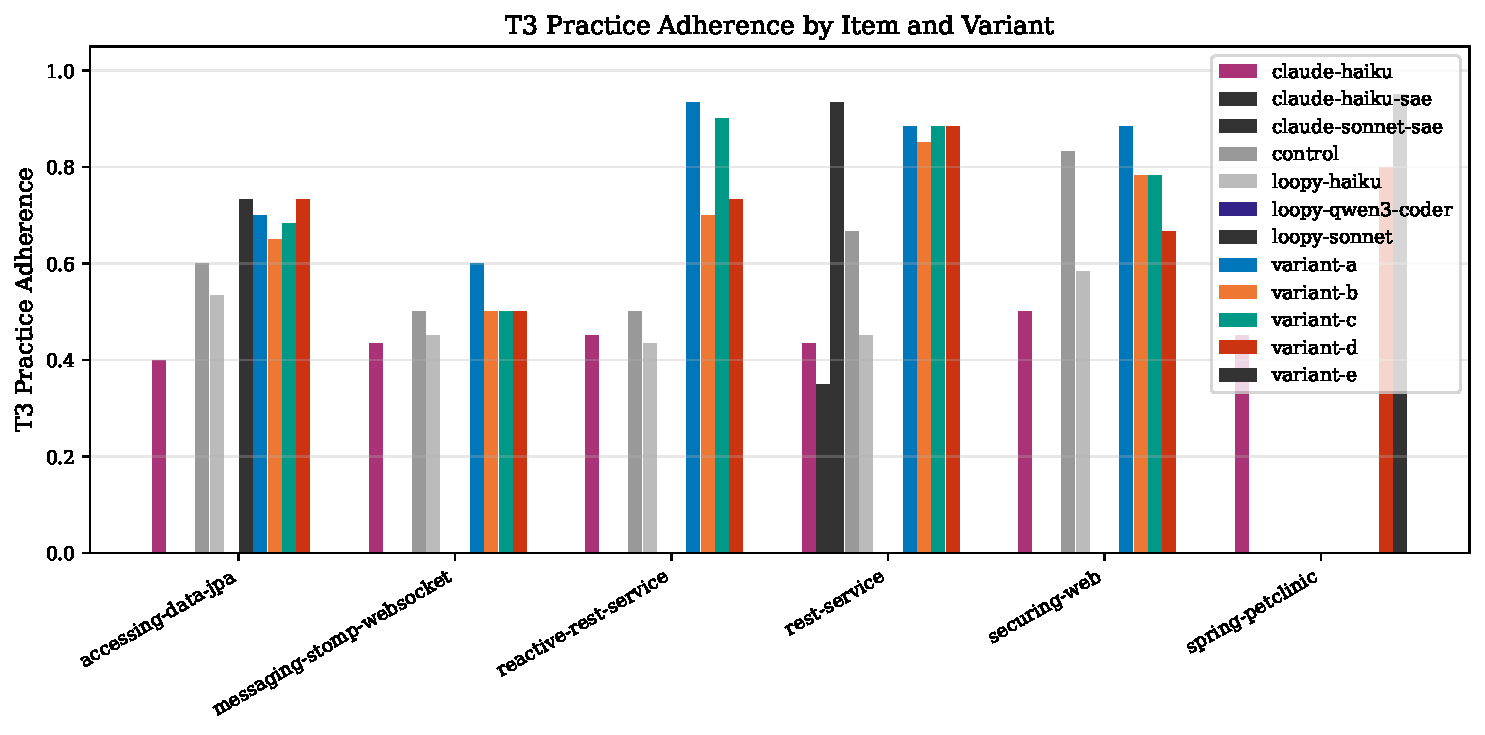
\includegraphics[width=0.9\textwidth]{figures/per-item-bars.pdf}
\caption{T3 practice adherence by item and variant.}
\end{figure}

\input{tables/per-item-breakdown}

%% ==================================================================
\section{Efficiency}

\input{tables/efficiency-breakdown}

\begin{figure}[H]
\centering
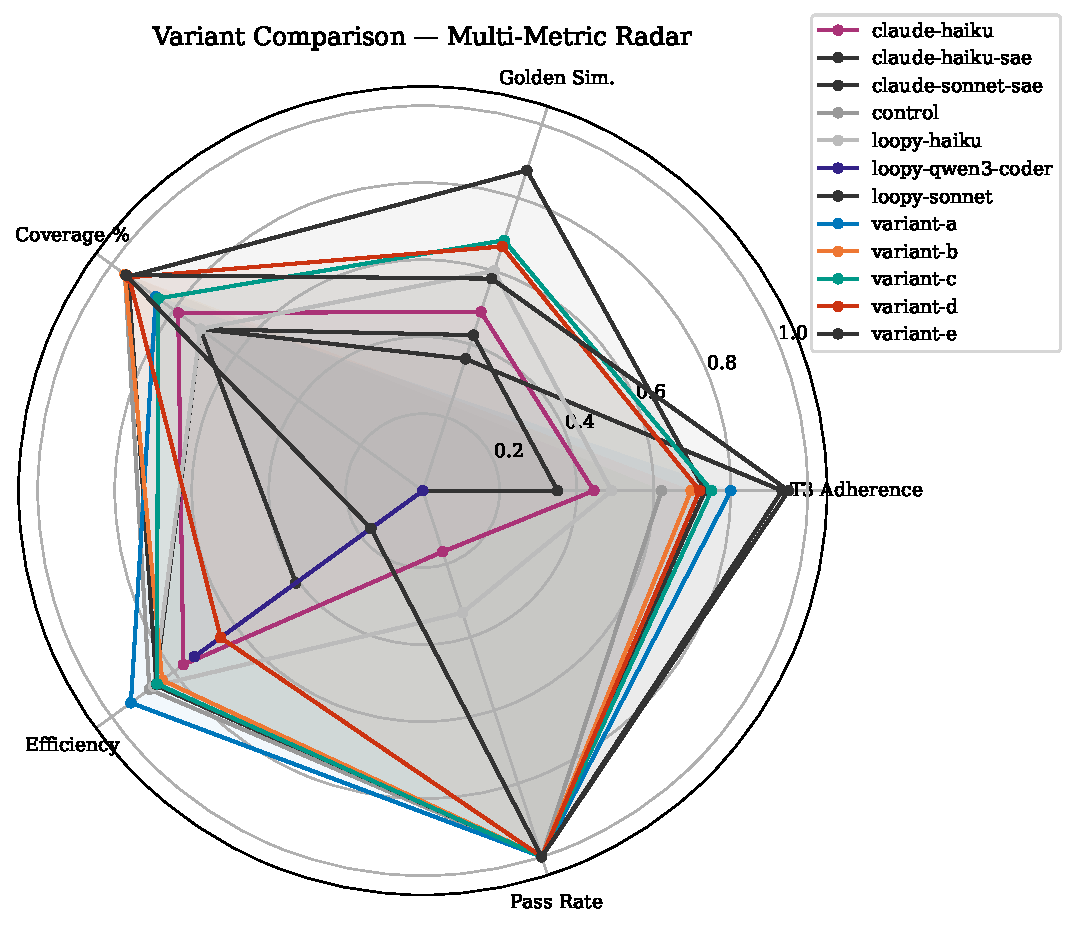
\includegraphics[width=0.8\textwidth]{figures/variant-radar.pdf}
\caption{Multi-metric radar chart across all variants.}
\end{figure}

%% ==================================================================
\section{Summary}

\begin{enumerate}
  \item \textbf{Prompt engineering is the biggest lever --- and the cheapest.}
        T3: 0.62 $\to$ 0.81. +29\% quality, same model.
  \item \textbf{Coverage lies.} 94\% coverage, T3=0.45. Without the jury you'd
        ship bad tests and never know.
  \item \textbf{There is a model floor.} Below it, no amount of tooling, knowledge,
        or prompting helps. Haiku, Qwen3 --- can't do it.
  \item \textbf{Model is the quality gate; framework is the cost gate.}
        Loopy:Sonnet (T3=0.73) $\approx$ CC:Sonnet (T3=0.70) --- same quality, 3$\times$ cost.
        The model determines \emph{whether it works}; the framework determines \emph{what it costs}.
  \item \textbf{Context compaction is the hidden cost multiplier.}
        Loopy without compaction: 18M input tokens. With compaction (threshold 0.3): 854K.
        21$\times$ reduction. Compaction tuning matters.
  \item \textbf{Knowledge amplifies capability --- it cannot create it.}
        Sonnet + SAE: T3=0.93. Haiku + SAE: T3=0.35. Same pre-computed analysis,
        opposite results.
  \item \textbf{Partial knowledge is worse than none.} Giving 3 files triggers
        more exploration than giving the full KB or nothing at all.
  \item \textbf{Structured execution shines on hard tasks.}
        Pet Clinic with plan/act: T3=0.95. Two-phase adds 2$\times$ cost on simple
        targets but pays off on complex ones.
\end{enumerate}

\end{document}
